\VSDMOEA{} is based on the principle of considering the diversity and stopping criterion in an explicit way, with the aim of altering gradually the optimization
search capabilities from exploration to exploitation.
%
This principle might be incorporated with any of the three categories of \MOEAS{}.
%
In this paper, our decision was to incorporate it in a dominance-based approach.
%
Particularly, our proposal considers the application of the fast-non-dominated-sort procedure so it might be considered as an extension
of \NSGAII{}~\cite{Joel:NSGAII}.
%
Also, it takes into account a more advanced way to control the diversity in the objective space.
%
%
%this modification, since the way of managing the objective space diversity have also been extended in several ways in \NSGAII{},
%Additionally, since the way in which \NSGAII{} preserve the diversity in the objective space  
%a more advanced way to control the diversity in the objective space was incorporated.
%
Overall, \VSDMOEA{} is a dominance-based \MOEA{} in which a novel replacement phase is provided,
i.e. no novel components are incorporated in the parent selection and variation stages.

\begin{figure}[t]
\centering
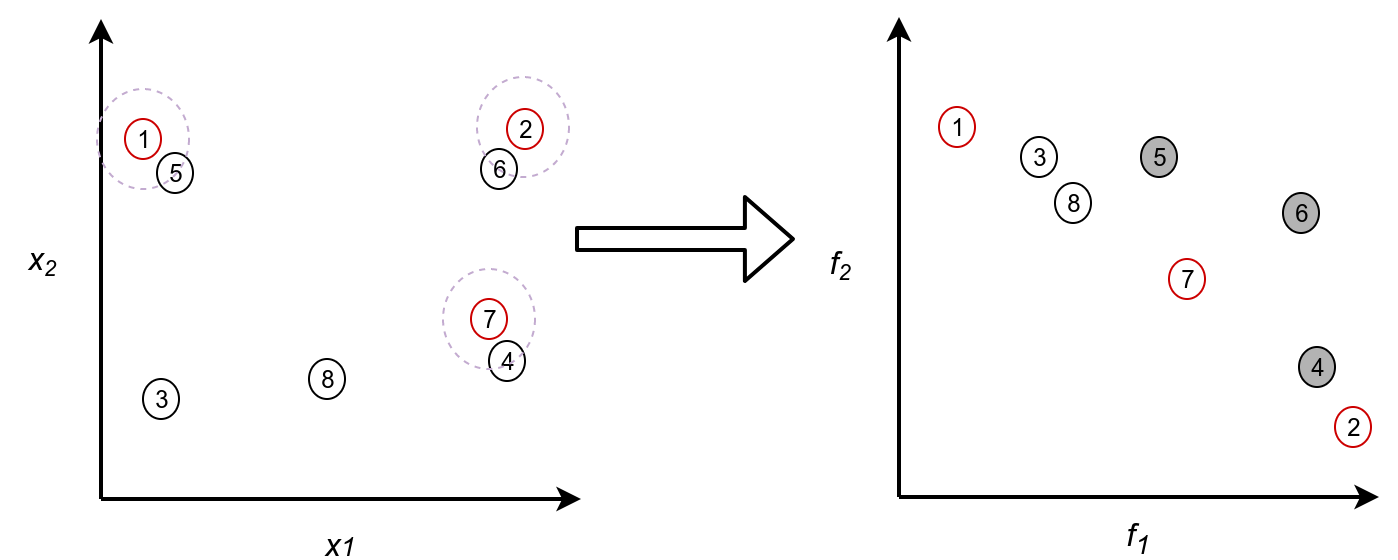
\includegraphics[width=0.45\textwidth]{Images/Fase_Remplazo_2.eps}
\caption{Replacement Phase - The left side represents the variables space and the right side the respectively objective space of the individuals.  }
\label{fig:Hypersphere}
\end{figure}


\subsection{Replacement Phase of VSD-MOEA}

The methodology used in the replacement phase considers some of the principles that were provided in the 
development of replacement phases for the single-objective domain~\cite{Joel:MULTI_DYNAMIC}.
%
%In these approaches, the offspring and parent individuals are joined to conform the parent of the next generation.
%and offspring individuals are joinethe individuals of the previous generation and offspring are joined to be selected.
%
In these approaches, at the begin of each generation the parents and offspring are joined.
%
Then, $N$ individuals must be selected to survive.
%
In order to take into account the diversity in the decision space, the 
Distance to Closest Neighbor (\DCN{}) is used.
%
In each step, this normalized distance (Eqn. \ref{eqn:distance}) is calculated with respect to those individuals that have already been selected to survive.
%
\begin{equation}\label{eqn:distance}
Distance(A, B) = \left (\sum_{i=1}^n \left ( \frac{A_i - B_i}{x_i^{(U)} - x_i^{(L)}} \right )^2  \right)^{1/2}
\end{equation}
Thus, individuals with large \DCN{} values are those that contribute in a significant way to preserve exploration in different regions of the search space.
%
In order to avoid an excessive decrease of the exploration degree, individuals with a \DCN{} value lower than a threshold value are penalized, meaning that
they are just selected if no non-penalized individuals exist.
%
In order to better visualize this principle, it can be considered that in each selection of a survivor, a hypersphere centered in such survivor is created.
%
Then, all the individuals that are inside a hypersphere are penalized.
%
One of the key novelties of the methodology is that the sizes of the hyperspheres are modified dynamically by taking into account the stopping criterion
and elpased generations.
%
Particularly, the sizes are decreased in a linear way, to alter the behaviour from exploration towards intensification.
%
Note that, this method requires a parameter which is the initial radius of the hyperspheres, which in this paper is denoted as $D_I$. 
%
A too large value might provoke the penalization of the whole set of individuals, meaning that a non-useful diversity might be maintained in the initial generations.
%
However, too small value might not penalize at all the individuals, meaning that the approach might behave as a traditional non-diversity based approach.

In order to better describe the principle of the replacement phase, we denote the individuals in the following way.
%
The \textit{reference individuals} are those that have been selected to survive to the next generation. 
%
The remaining ones are classified in \textit{penalized individuals} and \textit{candidate individuals}.
%
A representation of this scheme can be visualized in Fig.~\ref{fig:Hypersphere}.
%
The left part of the figure shows the decision space, whereas the right part is devoted to the objective space. 
%
The reference individuals are marked with a red border.
%
It can be visualized that surrounding each of them there is a circle with radius D (in dimensions larger than three it would be a hypersphere).
%
Then, any candidate individual that are inside a circle are penalized.
%
Penalized individuals are shown in grey in the right part.
%
Once that individuals are penalized, any of the typical approaches that are used to select survivors might be taken into account
by considering that penalized individuals do not exist.


\begin{algorithm}[t]
\algsetup{linenosize=\tiny}
  \scriptsize
	\caption{Replacement Phase of VSD-MOEA} 
\begin{algorithmic}[1]
\STATE Input: $P_t$ (Population of current generation), $Q_t$ (Offspring of current Generation)
    	\STATE Output: $P_{t+1}$
        \STATE $R_t = P_t \cup Q_t$
        \STATE $P_{t+1} = \emptyset$
        \STATE $Penalized = \emptyset$
				\STATE $D = D_I - D_I *2* \frac{G_{Elapsed}}{G_{End}}$ \label{DInicial} 			
		\STATE move( $R_t$,  $P_{t+1}$, Best in any of the objectives) 
        \label{alg:Extremos}
        \WHILE{ $|P_t|$ $\leq$ N }
			\STATE Compute \textbf{Diversity\_Variable\_Space} ($R_t$, $P_{t+1}$) \label{alg:Calculo_Diversidad_Primero}
		\STATE move($R_t$, Penalized, Variable space diversity $ < $ D)  \label{alg:Calculo_Diversidad_Primero_Move}
        \IF{$R_t$ is empty}
				\STATE Compute \textbf{Diversity\_Variable\_Space} ($Penalized$, $P_{t+1}$) \label{alg:Penalized_Diversity}
				\STATE move(Penalized, $R_t$, Largest variable space diversity) \label{alg:Penalized_Diversity_move}
        \ENDIF
		\STATE $conditionally-non-dominated-sort(R_t \cup P_{t+1}) $\label{alg:rank}
		\STATE Compute \textbf{Diversity\_Objective\_Space}($R_t$, $P_{t+1})$) \label{alg:Diversity_Space}
        \ENDWHILE
    	\RETURN $P_{t+1}$
	\end{algorithmic}
\label{alg:Replacement_Phase}
\end{algorithm}


The specific pseudocode of the replacement phase that is used in \VSDMOEA{} is shown in Algorithm~\ref{alg:Replacement_Phase}.
%
Basically, it is the approach previously described integrated with a procedure to meassure the contribution of each individual to the objective space.
%
In each step, the candidate individual with lowest rank and, in case of a tie, with the largest contribution to the diversity in the objective space is selected.
%
In each generation, the first step (line 3) is to join the parents ($P_t$) and the offspring ($Q_t$) in $R_t$.
%
Then, the set of penalized individuals and the next population are emptied (lines 4 and 5).
%
Additionally, the radius of the hyperspheres ($D$) is uptated (line 6).
%
Note that in the formula applied $D_I$ is the initial size of the hypersphere, $G_{Elapsed}$ is the amount of generations that have been evolved and $G_{End}$
is the stopping criterion, i.e. the number of generations that are to be evolved in the execution of \VSDMOEA{}.
%
It is clear that after half of the generations, the $D$ value is lower than 0, meaning that no penalties are performed.
%
This means that in the first half of the generations, more exploration than in traditional \MOEAS{} is induced, whereas 
in the final stages, a traditional \MOEA{} is applied.
%
The reason to induce such behaviour is that, we are not interested in obtaining a diverse set of solutions in the decision space at the end of the run.
%
Maintaining a diverse of solutions in the initial stages is just a way to promote exploration and reach a better Pareto front at the end of the execution.
%
Finally, the next population is filled with the boundary solutions, i.e. for each objective the best candidate solution is selected to survive (line 9).
%
Then, until $N$ individuals are selected (line 8), the following steps are carried out.
%
First, the \DCN{} value of each individual that has not been selected is calculated (line 9).
%
Then, those individuals with a \DCN{} value lower than $D$ are penalized (line 10).
%
If all the candidate individuals are penalized (line 11), it means that the amount of exploration is lower than expected.
%
Thus, the individual with largest \DCN{} values is recovered, i.e. moved to the non-penalized individuals set (line 12).
%
Finally, the objective space is taken into account.
%
Specifically, the candidate individuals and the reference set are joined.
%
Then, the fast-non-dominated-sort procedure is executed with such a set, stopping as soon as a front with a candidate individual is found (line 14).
%
Then, for each candidate individual that belongs to the lowest front, the individual with higher contribution to the diversity in the objective space is selected (line \ref{alg:Diversity_Space}).
%
The specific way in which the diversity in the objective space is measured is described in the next section.
%
%Particularly, if several candidates belong to the same front, the individual less crowded wins, similar principle that in the NSGA-II paradigm.
%
%Despite the fact that different diversity metrics are proposed in MOEAs, for simplicity in our proposal the objective space and variable space are guided with the DCN metric.
%
%However other diversity metrics can be implemented instead the DCN.

Note also that, as part of the diversity calculation of the variable space, a metric should be selected.
%
Since our experimental validation is performed with continuous domain, the normalized Euclidean distance is used.
%
However in discrete domains, other distance metrics such as the Manhattan, or the Hamming distance might be considered, and the definition of
such distance might affect the performance of the approach~\cite{Segura:17}.


%The main idea of replacement phase dwell in compute the contribution by each individual to diversity  in both spaces.
%
%Hence in each iteration just one individual is selected as survivor until the size of population is reached.
%
%Consequently this methodology separate the suitable candidates based in diversity of the variable space, afterward the best candidate in objective space is selected.
%

%
%The figure \ref{fig:Hypersphere} shows one iteration of the Replacement Phase where the reference individuals are $\{1, 2, 7\}$ and candidate individuals are $\{3, 4, 5, 6, 8\}$. 
%
%The individuals $\{4, 5, 6\}$ are moved to penalized set, since that each one is inside of a hypersphere (gray dotted circles) related to a reference individual.
%
%Finally, the candidate solutions are $\{2, 8\}$, due that both belongs to the same rank, the solution $8$ is selected since it has a better contribution to the diversity in the objective space.

%
%
%
%
% %The function definitions from algorithm~\ref{alg:Replacement_Phase} are explained as follow:
% %
% \begin{itemize}
% \item Diversity\_Variable\_Space(A,B): for each individual from set A an euclidean distance is computed in variable space to the closest solution from the set B.
% \item Diversity\_Objective\_Space(A,B): for each individual from set A an euclidean distance is computed in objective space to the closest solution from the set B.
%\end{itemize}
%
%
%

%ESto hay que moverlo a Experimental Validation
%Due that the initial diversity is influenced by  $D_I$ parameter, several experiments with different values have been realized.
%
%Accordingly that each dimension is normalized in the unity, the maximal hypersphere of the variable decisions is denoted by $\sqrt{N}$ where $N$ is the dimension of the variable space. 
%
%Under those circumstances, the hypersphere with radius $\sqrt{N}$ will cover outside from the bounds, for this reason it is multiplied by a factor $k$  resulting in the formula$D_I = k * \sqrt[]{N}  \rightarrow k \in (0,1)$.
%
%Empirically, the ideal configuration that provides quality solutions is $k=0.25$ .
%
%Additionally, the algorithm empirically is enough stable, given that different values of $k$ does not provide drastically differences in the solutions.


\subsection{Improvement distance in objective space}

Since the dominance definition is not related to the preservation of diversity in the objective space,
dominance-based \MOEAS{} incorporate special procedures to maintain diverse solutions.
%
Several different approaches have been defined, such as clustering and/or crowding with several different 
variants each of them.
%
In this paper, we define a novel distance metric, and then, as previously described a greedy approach, which selects an individual of the best front and with the largest distance.
%
Specifically, the novel distance is called ``Improvement Distance'' (ID) and it 
follows the same principles that guided the design of the IGD+ indicator~\cite{Joel:Inverted_Generational_Distance_Plus}.
%
The main idea is to prefer those individuals whose quality in all objectives is similarly preserved.
%
Particularly, a non-dominated individual can be very distant to the Pareto Front since that such individual could be the best in one objective but meaningly deteriorated in the rest of objectives, so as result it has high diversity in objective space.
%----
%The key idea is that, a direct Euclidean distance is used, those individuals that have very high values in some
%of the objectives might present very large distances which is not an adequate property.
%
In fact, high improvements in an objective value are related to larger selection probabilities and not the opposite, thus this behaviour should be avoided.
%
%In order to take this principle into account, when calculating the distance between two individuals

The key idea considers the dominance relation between the candidate and reference individuals. % when the distance is computed.
%
%
Consequently, a reference and a candidate individuals are compared.
%
If the candidate individual is dominated by the reference individual, then the euclidean distance with no modification is implemented.
%
However if they are non-dominated with each other, then is calculated the minimum distance from the reference point to the dominated region by the candidate individual. %
This distance can be viewed as an amount of inferiority of the solution in comparison with the reference individual.	
%
The improvement distance is defined in (\ref{eq:ImprovementDistance}) where $R$ and $C$ are the reference and candidate solutions respectively. 
\begin{equation} \label{eq:ImprovementDistance}
ID(R, C) = \left (\sum_{i=1}^M \left (max(0, R_i - C_i \right ))^2  \right)^{1/2}
\end{equation}
Specifically, this distance is considered as a Weakly Pareto Compliant Indicator.
%
In addition, this metric relaxes some difficulties encountered when the number of objectives is increased, given that the solutions in many objectives are usually non-dominated with each other by using the Pareto dominance relation.
%
This means a very low selection pressure toward the Pareto front in Pareto-dominance-based MOEAS \cite{Joel:Optimization_Of_Scalarizing_Functions_Through_Evolutionary_MOEAS}.
%
Principally, the improvement distance is effective with over-prioritization  of dominance-resist solutions i.e., solutions with exceptional performance in one objective and extremely poor performance in many others \cite{Joel:Failure_MOEAs}.
%


Through the literature several crossover operators have been proposed in MOEAs~\cite{Joel:ParentMeanCentricSelfAdaptation},  
a popular operator is the Simulated Binary Crossover (SBX).4\cite{Joel:SBX1994}%, Joel:TAXONOMY_CROSSOVER, Joel:Kalyanmoy}
%	
In addition based in diversity-related properties the No-Reflection Dynamic SBX is implemented \cite{Joel:DNR_SBX}, which is considered as a variant of the SBX operator.


